\documentclass[11pt]{article}

\usepackage{color} 
\usepackage{graphics}
\usepackage{graphicx}
\usepackage{pstricks}
\usepackage{listings}% http://ctan.org/pkg/listings
\lstset{
  basicstyle=\ttfamily,
  mathescape
}

\title{\textsf{molsim} tutorial \\ \bigskip \tiny{for the v. 0.9 series}}
\author{J.S. Hansen}
\date{Februaray 2022}
  
\begin{document}

\maketitle

\section{Introduction}

\textsf{molsim} is a GNU Octave/Matlab toolbox for molecular dynamics
simulations. \textsf{molsim} supports simulations of
\begin{itemize}
\item simple Lennard-Jones systems,
\item molecular systems with bond, angle, and torsion potentials, 
\item confined flow systems, eg., Couette and Poiseuille flows,
\item charged systems using shifted force and Wolf methods,
\item dissipative particle dynamics systems,
\item different ensembles, 
\item and more \ldots
\end{itemize}

\bigskip
\noindent \textsf{molsim} is basically a wrapper for the \textsf{seplib}
library, which is a light-weight flexible molecular dynamics simulation library
written in ISO-C99. \textsf{seplib} is CPU-based and offers shared memory
parallization; this parallizaton is supported by
\textsf{molsim}. \textsf{seplib} is also developed and maintained by this
author, and the underlying algorithms are based on the books by Allen and
Tildesley \cite{AllenTildesley}, Frenkel and Smit \cite{FrenkelSmit}, Rapaport
\cite{Rapaport}, and Sadus \cite{Sadus}.

\bigskip
\noindent In this text
\begin{verbatim}
>> 
\end{verbatim}
symbolizes the GNU Octave/Matlab command prompt. This 
\begin{verbatim}
$ 
\end{verbatim}
symbolizes the shell prompt.

\bigskip
\noindent Example scripts and functions to simulate different systems can be
found under the package \textsf{tests} directory. It is highly recommended that
the user's project starts from one of these \textsf{.m}-files, and the user
then makes the necessary changes.  

\section{Installation}
\subsection{GNU Octave}
GNU Octave's package manager offers a very easy installation. From the command
prompt type (one single line)
\begin{verbatim} 
>> pkg install "https://github.com/jesperschmidthansen/molsim/archive/ \
                                             refs/tags/v<version>.tar.gz"
\end{verbatim}
to install the package. \verb!<version>! can be for example \verb!0.9.2!. Check
contact to \verb!molsim! by
\begin{verbatim}
>> molsim('hello')
Hello. 
\end{verbatim}
You can also download the \verb!tar.gz! file manually from
\begin{verbatim}
https://github.com/jesperschmidthansen/molsim
\end{verbatim}
and save it in some directory of your choice. From this directory enter GNU
Octave and type
\begin{verbatim}
>> pkg install molsim-<version>.tar.gz 
\end{verbatim}
    
\subsection{Matlab}
From
\begin{verbatim}
https://github.com/jesperschmidthansen/seplib/
\end{verbatim}
\noindent download and save the current release \verb!seplib-<version>.tar.gz!
in a directory of your choice. Unpack, configure and build the library
\begin{verbatim}
$ tar zxvf seplib-<version>.tar.gz
$ cd seplib
$ ./configure
$ make
$ cd octave
\end{verbatim}
To build the \textsf{mex}-file enter Matlab
\begin{verbatim}
$ matlab -nodesktop
\end{verbatim}
and run the script \verb!buildmex!, that is, 
\begin{verbatim}
>> buildmex
\end{verbatim}
Depending on the system this will build a \verb!molsim.mex<archtype>!  file;
\verb!<archtype>! being your computer architecture. Copy this file to a
directory in your Matlab search path.

\bigskip

\noindent Note: Matlab compatibility is not guarantied. \textsf{molsim} will
only be tested against very limited Matlab versions.

\section{The interface strategy}
This tutorial is not meant to introduce molecular dynamics; such introduction
can be found in the books listed in the reference list. In brief, the basic idea
is to solve the classical equation of motion of an ensemble of interacting
particles. In the simplest form this means solving (numerically) Newton's second
law
\begin{equation}
  \frac{\mathrm{d}\mathbf{r}_i}{\mathrm{d} t} = \mathbf{v}_i \ , \ \
  \frac{\mathrm{d}\mathbf{p}_i}{\mathrm{d} t} = \mathbf{f}_i
\end{equation}
where $\mathbf{r}_i, \mathbf{v}_i, \mathbf{p}_i$ and $\mathbf{f}_i$ are the
particle position, velocity, momentum and force acting on the particle, respectively. In a
standard simulation we solve this set of differential equations by (i)
evaluating the forces acting on the particles, and (ii) from this integrate
forward in time. The following pseudo code lists the basic idea

\bigskip

\clearpage

\noindent \textbf{Listing 0}
\begin{lstlisting}
Set simulation parameters
Set initial configuration $\mathbf{r}, \mathbf{p}$

do (as many times as we want)
   $\mathbf{f}$ $\leftarrow$ calcforce($\mathbf{r}$)
   $\mathbf{r},\mathbf{p}$ $\leftarrow$ integrate($\mathbf{f}$,$\mathbf{p}$)
done
\end{lstlisting}
---

\noindent The \textsf{molsim} interface seeks to emulate this, and give the user
coding flexibility and accessibility to the simulation quantities. In general,
the \verb!molsim! interface is on the form
\begin{verbatim}
molsim(<action>, <specifier>, <arguments>);
\end{verbatim}
The action can be any particular action the user wishes to perform, for example,
\verb!calcforce!, \verb!integrate!, and so on. The action is specified by the
second argument; say, \verb!lj! specifies that action \verb!calcforce! should
apply the Lennard-Jones interaction. The specifier arguments are given in the
final input and can be a scalar, string, vector, or a sequence of these.

\section{First quick example: The Lennard-Jones liquid}
Listing 1 shows a script simulating a standard Lennard-Jones (LJ) system in the
micro-canonical ensemble, where number of particles, volume, and total
mechanical energy is conserved.

\bigskip

\noindent \textbf{Listing 1}
\begin{verbatim}
% Specify the LJ parameters
cutoff = 2.5; epsilon = 1.0; sigma = 1.0; aw=1.0;

% Set init. position and velocities 10x10x10 particles 
% in box with lengths 12x12x12. Velocities set to default. 
% Configuration stored in start.xyz. 
molsim('set', 'lattice', [10 10 10], [12 12 12]);

% Load the configuration file
molsim('load', 'xyz', 'start.xyz');

% Main mol. simulation loop - 10 thousand time steps
for n=1:10000

  % Reset forces etc
  molsim('reset');

  % Calculate force between particles of type A (default type)
  molsim('calcforce', 'lj', 'AA', cutoff, sigma, epsilon, aw);

  % Integrate forward in time - use leapfrog alogrithm
  molsim('integrate', 'leapfrog');
 
end

% Free memory allocated
molsim('clear');
\end{verbatim}
---

\noindent In Listing 1 no information is printed or saved, and, admitted, not very
useful. Inside the main loop the user can call the \textsf{print}-action, for
example, 
\begin{verbatim}
if rem(n,100)==0
  molsim('print');
end
\end{verbatim}
to print current iteration number, potential energy per particle, kinetic energy
per particle, total energy per particle, kinetic temperature, and total momentum
to screen every 100 time step.

Information can also be stored into variables for further analysis. For example,
to get the system energies and pressure
\begin{verbatim}
[ekin, epot] = molsim('get', 'energies');
press = molsim('get', 'pressure');
\end{verbatim}
and particle positions and velocities
\begin{verbatim}
x = molsim('get', 'positions');
v = molsim('get', 'velocities');
\end{verbatim}
In the reference sheet (see Appendix) you can find the list of
specifiers for the \verb!get! action.

\textbf{IMPORTANT NOTE} For molecular systems the pressure is
calculated using the molecular pressure tensor. In general this is different
from the atomic pressure. The user must enable this calculation using the
\verb!set! action with specifier \verb!molstresscalc!. For example, to
calculate the (molecular) pressure every ten time step use
\begin{verbatim}
molsim('set', 'molstresscalc', 10);
\end{verbatim}
Then in the main loop retrieve the pressure
\begin{verbatim}
if rem(n,10)==0
  [press_atomic, press_mol]=molsim('get', 'pressure');
end
\end{verbatim}

\subsection{NVT and NPT simulations}
Often you will not perform simulations in the micro-canonical ensemble, but
under a desired temperature and/or pressure. One way to achieve this with
\verb!molsim! is to use simple relaxation algorithms. To simulate at
temperature, say 2.2, you call the action \verb!'thermostat'! with specifier
\verb!'relax'! after the integration step
\begin{verbatim}
molsim('thermostat', 'relax', 'A', 2.2, 0.01);
\end{verbatim}
The last argument is the relaxation parameter; the higher value the faster
relaxation. Notice that too large values make the system unrealistically
stiff; the best value is optimized via trail-and-error. There is also a
Nos\'{e}-Hoover thermostat available with the interface
\begin{verbatim}
molsim('thermostat', 'nosehoover','A' ,2.2, 10.0);
\end{verbatim}
The last argument is here the thermostat mass and not the relaxation
time. Again, you should choose this parameter with care.

To simulate at pressure, say 0.9, you call the action \verb!'barostat'! after
the integration step,
\begin{verbatim}
molsim('barostat', 'relax', 0.9, 0.01, 'iso');
\end{verbatim}
The choice of relaxation parameter, here 0.01, is again a matter of the specific
system. The last argument tells the barostat to do an isotropic compression. If
this is left out the barostat works by changing the system box length in the
$z$-direction only (an-isotropic scaling); this is practical when doing sampling
as two directions are fixed. You can use the barostate and the thermostat
in the same simulation mimicking an NPT system. For the expert: The barostat is
based on the atomic pressure, a molecular pressure barostat is planned for
future releases.  

\section{The \textsf{molsim} force field}
\verb!molsim! supports simulations of more complicated systems. In general, the
\textsf{molsim} force field is defined from the potential function
\begin{equation}
  U(\mathbf{r}_i, r_{ij}, \ldots)
  =  U_\mathrm{lattice} + U_\mathrm{vWaals} + U_{\mathrm{coulomb}} +
  U_\mathrm{bonds} + U_\mathrm{angles} + 
  U_\mathrm{torsion}
\end{equation}
The first term allows for simulations of fictitious fixed crystal arrangements,
where the particles/atoms are tethered around a pre-set lattice site. This is
particular useful for systems with walls. The potential function is a harmonic
spring type
\begin{equation}
  U_\mathrm{lattice} =
  \sum_\mathrm{sites} \frac{1}{2}k_0 (\mathbf{r}_i - \mathbf{r}_0)^2 \ ,
\end{equation}
where $k_0$ is the spring constant, $\mathbf{r}_i$ is the position of
particle/atom $i$, and $\mathbf{r}_0$ is the virtual lattice site. Using this
requires that the virtual crystal sites are set: use
\verb!molsim('set','virtualsites');! to set the current positions as crystal
sites. The force from this potential is calculated by
\begin{verbatim}
molsim('calcforce', 'lattice', <part. type>, <k0>);
\end{verbatim}
where \verb!<part. type>! is the particle type and \verb!<k0>! is the force
constant. 

The short ranged van der Waals pair interaction is given via the 12-6 
Lennard-Jones potential
\begin{equation}
  U_\mathrm{vWaals} =  \sum_{i,j \, \mathrm{pairs}}
  4\epsilon\left[\left(\frac{\sigma}{r_{ij}}\right)^{12} - a_w
    \left(\frac{\sigma}{r_{ij}}\right)^{6}\right] \, .
\end{equation}
Here $r_{ij}$ is the particle distance, $\epsilon$ and $\sigma$ define the
characteristic energy and length scales. The parameter $a_w$ determines the
weight of the attractive second term in the potential function. The force call
is
\begin{verbatim}
molsim('calcforce', 'lj', <pair>, <cutoff>, <sigma>, <eps>, <aw>);
\end{verbatim}
where \verb!<cutoff>! is the maximum interaction length (or cut-off). This must
be less than or equal to the maximum system interaction length which is by
default 2.5. The system maximum interaction length can be set via the
\verb!set! action
\begin{verbatim}
molsim('set', 'cutoff', <value>);
\end{verbatim}

The Coulomb potential is 
\begin{equation}
  U_{\mathrm{coulomb}} = \sum_{i,j \, \mathrm{pairs}}\frac{q_iq_j}{r_{ij}} \, .
\end{equation}
Currently this long ranged interaction is evaluated using approximate
shifted-force or Wolf methods; this can be specified. Note: these two
algorithms do not apply to confined systems. The call is
\begin{verbatim}
molsim('calcforce', 'coulomb', <method>, <cutoff>, <optWolf>);
\end{verbatim}
\verb!<method>! can take value \verb!'sf'! or \verb!'wolf'!, and
\verb!<optWolf>! is the Wolf screening parameter which must be specified if the
Wolf method is chosen. Again, the cut-off must be less than or equal to the
maximum system interaction length.

Bonds are model via the harmonic spring potential
\begin{equation}
  U_{\mathrm{bonds}} =\sum_{\mathrm{bonds}} \frac{1}{2} k_{s}(r_{ij} - l_0)^2 \, .
\end{equation}
$k_s$ is the spring constant and $l_0$ is the zero force bond length. 
Currently \textsf{molsim} does not support rigid bonds. To calculate the force
from bonds use
\begin{verbatim}
molsim('calcforce', 'bond', <type>, <ks>);
\end{verbatim} 
\verb!<type>! specifies the specific bond type. Bond, angle, and torsion angle
types are specified through integers, see example script later. 

The angle potential is the cosine squared potential
\begin{equation}
  U_{\mathrm{angles}}=\frac{1}{2}\sum_{\mathrm{angles}} k_{\theta} (\cos(\theta) - \cos(\theta_0))^2 \, ,
\end{equation}
where $k_\theta$ is the force amplitude, and $\theta_0$ the zero-force
angle. See Fig. \ref{fig:torsion} for the angle definition. The call is
\begin{verbatim}
molsim('calcforce', 'angle', <type>, <a0>, <ka>);
\end{verbatim}
where \verb!<type>! specifies the angle type, \verb!<a0>! the zero force angle,
$\theta_0$, and \verb!<ka>! the force constant, $k_\theta$.  
\begin{figure}[h]
  \begin{center}
    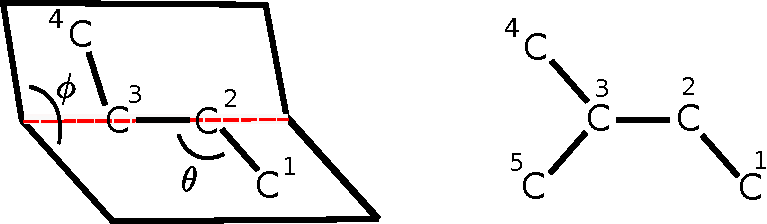
\includegraphics[scale=.7]{diheadral.pdf}
  \caption{
    \label{fig:torsion}
    Illustration of the angle and torsion angle.
  }
  \end{center}
\end{figure}

Finally, the torsion angle potential is the Ryckaert-Belleman potential 
\begin{equation}
  U_\mathrm{torsion}=\sum_{\mathrm{angles}} \sum_{n=0}^5 c_n
  \cos^n(\pi-\phi)
   \, . 
\end{equation}
Here $c_n$ are the six Ryckaert-Belleman coefficients, and $\phi$ is the
torsion angle, see Fig. \ref{fig:torsion}. Two illustrative 
examples are when only $c_1 \neq 0$:
\begin{enumerate}
\item If $c_1 > 0$ then the minimum energy torsion angle is $\phi = 0$; this is
  illustrated in the right-hand figure of a planar molecule with the torsion
  angle defined by the 1-2-3-5 bonds. 
\item If $c_1 < 0$ then the minimum energy torsion angle is $\phi = \pi$; this
  is the torsion angle defined by the 1-2-3-4 bonds. 
\end{enumerate}
To calculate the force from this interaction potential use
\begin{verbatim}
molsim('calcforce', 'torsion', <type>, <RB-coef>);
\end{verbatim}
\verb!<RB-coef>! is an array of length six specifying the Ryckert-Belleman
coefficients. Note, the torsion angle is often referred to as the diheadral angle. 

\section{Molecular systems: Toluene}
This example shows how to setup a simulation of model liquid toluene. The model
of the molecule is a so-called united atomic unit (UAU) model. This means that
each carbon group is represented by a single Lennard-Jones particle, thus, the
toluene molecule is composed of seven identical Lennard-Jones particles, six
forming the phenyl ring structure (particle indices 2-7) and one representing
the methyl group (index 1).  We exclude the molecular dipole moment, i.e., we do
not apply any charges to the system. The model molecule is shown in
Fig. \ref{fig:toluene}.
\begin{figure}[h]
  \begin{center}
    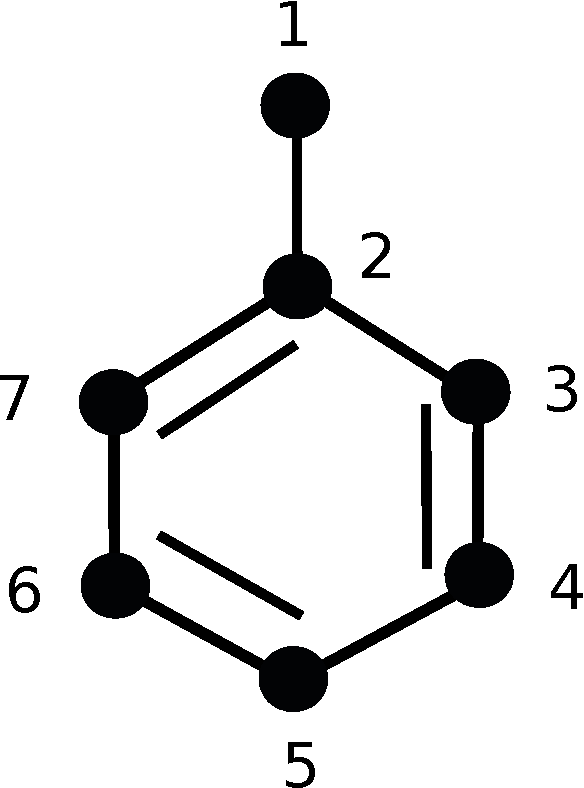
\includegraphics[scale=.4]{toluene.pdf}
  \caption{
    \label{fig:toluene}
    United atomic unit representation of toluene.
  }
  \end{center}
\end{figure}

To define the molecule geometry (or topology) we need different intra-molecular
interactions, i.e., bond, angle, and torsion angle potentials. Lennard-Jones
interactions between carbon groups in same molecule are excluded. The model is
further simplified by using only two different bond types (with different zero
force bond length, but same force constant), and one angle type. There are two
different torsion angles, eg., 1-2-3-4 form one type of torsion angle,
$\phi=\pi$, whereas 7-2-3-4 form torsion angle with $\phi=0$. We define the
molecular model in two files; one with extension \verb!.xyz! giving the carbon
groups' positions for one molecule and one with extension \verb!.top!  defining
bonds and angles in the molecule. You can find examples of these two files for
different molecules under the \verb!resources!  directory.

To setup the entire system (i.e. the ensemble of molecules) we copy the single
molecule \verb!.xyz!  and \verb!.top! to the current directory and use the
\verb!set!  action; for example to simulate 500 molecules
\begin{verbatim}
>> molsim('set', 'molconfig', 'toluene.xyz', 'toluene.top', ... 
   500, 0.05, 42)
\end{verbatim}
The two last arguments are the molecular number density (keep very low initially
and compress the system afterwards), and a seed for the random number
generator. This generates a system \verb!start.xyz! file and \verb!start.top!
file that can be loaded by your program. 

We now only need the parameter values for the interaction potentials and we will
simply use what is available in the literature \cite{Hansen} and convert them
into MD reduced units. Listing 2 shows the resulting script

\bigskip

\noindent \textbf{Listing 2}
\begin{verbatim}
% Simulation parameters 
% (Corresponds to 298.15 K, 862 kg/m^3)
temp0 = 4.969; dens0 = 1.96; dt  = 0.001; nloops = 200000;

% Intra-molecular parameters
bondlength_0 = 0.4; bondlength_1 = 0.38; springconstant = 48910;
bondangle = 2.09; angleconstant = 1173;

torsionparam_0 = [0.0, 133.0, 0.0, 0.0, 0.0]; 
torsionparam_1 = [0.0, -133.0, 0.0, 0.0, 0.0];

% Load positions, set temp, remove intra-molecular pair-interaction etc
molsim('load', 'xyz', 'start.xyz');
molsim('load', 'top', 'start.top');

molsim('set','timestep', dt);
molsim('set', 'temperature', temp0);
molsim('set', 'exclusion', 'molecule');

% Main loop
for n=1:nloops
  molsim('reset')

  molsim(’calcforce’, ’lj’, ’CC’, 2.5, 1.0, 1.0, 1.0);
  
  molsim(’calcforce’, ’bond’, 0, bondlength_0, springconstant);
  molsim(’calcforce’, ’bond’, 1, bondlength_1, springconstant);
  
  molsim(’calcforce’, ’angle’, 0, bondangle, angleconstant);

  molsim(’calcforce’, ’torsion’, 0, torsionparam_0);
  molsim(’calcforce’, ’torsion’, 1, torsionparam_1);
  
  molsim('thermostate', 'nosehoover', 'C', temp0, 10.0);
  molsim('integrate', 'leapfrog');

  molsim('compress', dens0);

end
\end{verbatim}

\noindent ---

\noindent Notice that
\begin{itemize}
\item \verb!molsim('set', 'exclusion', 'molecule');! ensures that van der Waals
  (and in general also the Coulomb) interactions are excluded if the particles
  are in same molecule. Exclusion can also be set for bonded particles using the
  'bond' argument.
\item For the \verb!bond!, \verb!angle!, and \verb!torsion! specifiers the first
  argument pertains to the type.  
\end{itemize}

\section{Sampling}
The user can access the system configuration through the \verb!get! action and
from this perform data analysis via GNU Octave's or Matlab's built-in
tools. \textsf{molsim} also offers some run-time data sampling. The different
samplers are initialized before the main loop using the \verb!sample!-action
\begin{verbatim}
molsim('sample', <sample specifier>, <arguments>);
\end{verbatim}
For example, to sample the stress autocorrelation function with 200 sample points
and over a sample time span window of 5.0 we write
\begin{verbatim}
molsim('sample', 'sacf', 200, 5.0);
\end{verbatim}
The actual sampling is carried out by the specifier \verb!do!; inside the main
loop there must be one call
\begin{verbatim}
molsim('sample', 'do'); 
\end{verbatim}
Typically this call is done just after the integration. Check the reference
sheet for the list of available samplers. 

\section{Parallization}
\textsf{molsim} offers two types of sheared memory parallization, namely,
\begin{itemize}
\item Loop parallization 
\item Task-block parallization
\end{itemize}
We here only document the first type\footnote{Yep - I'm lazy}; the task-block
type will be included in later versions of the tutorial. To use loop
parallization simply call the \verb!set! action with specifier \verb!omp!
\begin{verbatim}
molsim('set', 'omp', <nthreads>);
\end{verbatim}
where \verb!nthreads! is the number of threads you wish to use. Typically, do
not use more threads than the number of cpu-cores\footnote{not even with
  hyper-threading}.  The call is placed anywhere before the main loop. Be aware
that depending on your hardware and the particular system the parallization
efficiency quickly drops as function of number of threads. To explore this we
define the speed-up and efficiency by
\begin{equation}
  \mathrm{speedup} = \frac{t_\mathrm{single}}{t_\mathrm{parallel}} \ \
  \mathrm{and} \ \ 
  \mathrm{efficiency} = \frac{t_\mathrm{single}}{t_\mathrm{parallel}
    N_\mathrm{threads}}
  \, ,
\end{equation}
where $t_\mathrm{single}$ is the single thread execution time and
$t_\mathrm{parallel}$ the parallel execution time. The speed-up is plotted in
Fig. \ref{fig:bench} for a simple Lennard-Jones liquid simulation.
\begin{figure}[h]
  \begin{center}
    \includegraphics[scale=.4]{speedup.eps}
  \caption{
    \label{fig:bench}
    Left: Speed-up as function of number of threads. Right: Efficiency as
    function of number of threads. The test machine is a 72-core machine.
  }
  \end{center}
\end{figure}
The efficiency is also plotted in Fig. \ref{fig:bench}. The efficiency quickly
drops, even on this multi-core machine, and adding more threads (using more cpu
cores) is not always optimal. In the \verb!tests!-directory you can find
\verb!molsim_runparallel.m! that times the execution time for a given system
size, density and number of threads; use the \verb!help! command for its usage.

\bigskip

\noindent

\begin{thebibliography}{9}

\bibitem{AllenTildesley}
  M. P. Allen and D. J. Tildesley, \emph{Computer Simulation of Liquids}, (1989). 

\bibitem{FrenkelSmit}
  D. Frenkel and B. Smit, \emph{Understanding Molecular Simulation}, (1996).

\bibitem{Rapaport}
 D. C. Rapaport, \emph{The Art of Molecular Dynamics Simulation}, (1995).

\bibitem{Sadus}
  R. J. Sadus, \emph{Molecular Simulation of Fluids. Theory, Algorithms and
    Object-Orientation}, (1999).

\bibitem{Hansen}
  J.S. Hansen \emph{Where is the hydrodynamic limit?} Mol. Sim., 47:1391 (2021).
\end{thebibliography}

\appendix

\clearpage

\begin{center}

  {\huge{Reference sheet}}
  
  \bigskip

  \bigskip
  
  \begin{tabular}{cclclcccc}
    {\color{red}{\textbf{Action}}} && {\color{blue}{Specifier}} && Arguments && Output \\
                                   && && && \\
    \hline
                                   && && && \\
    \verb!load! && \verb!xyz! && file name && \\
    $\mbox{}$ && \verb!top! && file name && \\
                                   && && && \\
    \hline
    && && && \\
    \verb!save! &&  && 1: type names && \\
                &&  && 2: file name && \\
                                   && && && \\
    \hline
                                   && && && \\
    \verb!set! && \verb!timestep! && time step (0.005) && \\
    $\mbox{}$  && \verb!temperature! && temperature (1.0) && \\
    $\mbox{}$  && \verb!cutoff! && Max. cut-off (2.5) && \\
    $\mbox{}$  && \verb!omp! && No. of threads && \\
    $\mbox{}$ && \verb!exclusion! && 'bond' or 'molecule' && \\
    $\mbox{}$ && \verb!temperaturerelax! && relaxation time (0.01) && \\
    $\mbox{}$ && \verb!compressionfactor! && compress factor (0.9999) && \\
    $\mbox{}$ && \verb!types! && particles types (vector string) && \\
    $\mbox{}$ && \verb!skin! && buffer-skin neighblist && \\
    $\mbox{}$ && \verb!charges! && atom charges (vector) && \\
    $\mbox{}$ && \verb!lattice! && 1: array [$N_x , N_y , N_z$] && \\
    $\mbox{}$ && $\mbox{}$      && 2: array [$L_x, L_y, L_z$] && \\
    $\mbox{}$ && \verb!molconfig!&& 1: \textsf{xyz} file && \\
              &&                 && 2: \textsf{top} file && \\
              &&                 && 3: No. molecules && \\
              &&                 && 4: Crystal density && \\
              &&                 && 5: Random seed && \\
              &&\verb!virtualsites!&& && \\
    $\mbox{}$ &&\verb!molstresscalc! && iterations between calculation && \\ 
    && && && \\
    \hline                                           
  \end{tabular}

\end{center}

\begin{center}
  
  \begin{tabular}{cclclclll}
    {\color{red}{\textbf{Action}}} && {\color{blue}{Specifier}} && Arguments && Output \\
                                   && && && \\
    \hline
                                   && && && \\
    \verb!get! && \verb!numbpart!&& && scalar\\
    $\mbox{}$  && \verb!box! && && 3-vector \\
    $\mbox{}$  && \verb!energies! && && 2-vector (kin, pot)\\
    $\mbox{}$  && \verb!pressure! && && scalar(s) (p, pmol) \\
    $\mbox{}$  && \verb!velocities! && && $N_\mathrm{part.}\times 3$-matrix \\
    $\mbox{}$  && \verb!positions! && &&  $N_\mathrm{part.}\times 3$-matrix \\
    $\mbox{}$  && \verb!forces! && &&  $N_\mathrm{part.}\times 3$-matrix \\
    $\mbox{}$  && \verb!types! && && $N_\mathrm{part.}$-string \\
    $\mbox{}$  && \verb!mass! && && $N_\mathrm{part.}$-vector \\
    $\mbox{}$  && \verb!charges! && && $N_\mathrm{part.}$-vector \\
    $\mbox{}$  && \verb!molpositions! && && $N_\mathrm{mol}\times 3$-matrix \\
    $\mbox{}$  && \verb!molvelocities! && && $N_\mathrm{mol}\times 3$-matrix \\
    $\mbox{}$ && \verb!indices! && && $N_\mathrm{uau}$-vector \\
    $\mbox{}$ && && && \\
    \hline
                                   && && && \\
    \verb!calcforce! && \verb!lj! && 1: part. types && \\
                                   && && 2: cutoff&& \\
                                   && && 3: $\sigma$ && \\
                                   && && 4: $\epsilon$ && \\
                                   && && 5: $a_w$ && \\
                  &&\verb!coulomb!&& 1: method && \\
                                   && && 2: cutoff && \\
                                   && && 3: opt. Wolf param.\\
                    && \verb!bond! && 1: type && \\  
                    &&             && 2: bond length && \\
                    &&             && 3: spring constant && \\
                    && \verb!angle!&& 1: type && \\  
                    &&             && 2: zero angle force && \\
                    &&             && 3: force constant && \\            
                    && \verb!torsion! && 1: type && \\  
                    &&             && 2: tors. param && \\
                    && \verb!lattice! && 1: part. type && \\
                    &&               && 2: spring constant && \\   
                    && \verb!dpd! && 1: part. types && \\
                    &&            && 2: cutoff && \\  
                    &&            && 3: rep. parameter && \\ 
                    &&            && 4: $\sigma$ && \\
                                   && && && \\
    \hline
    && && && 
  \end{tabular}

\end{center}


\clearpage
\begin{center}
  
  \begin{tabular}{cclclclll}
    {\color{red}{\textbf{Action}}} && {\color{blue}{Specifier}} && Arguments && Output \\
                                   && && && \\
    \hline
                                   && && && \\
    \verb!integrate! && \verb!leapfrog! && && \\
    $\mbox{}$ && \verb!dpd!      && $\lambda$ && \\
                                   && && && \\
    \hline
                                   && && && \\
    \verb!thermostat! && \verb!relax! && 1: type && \\
    $\mbox{}$   &&       && 2: target temperature && \\
    $\mbox{}$  &&        && 3: relax time && \\
    $\mbox{}$  && \verb!nosehoover! && 1: type && \\
    $\mbox{}$  &&            && 2: target temperature && \\
    $\mbox{}$  &&            && 3: themostate mass && \\
                                   && && && \\
    \hline
                                   && && && \\
    \verb!barostat! && \verb!relax! && 1: target pressure && \\
    $\mbox{}$   &&       && 2: relax time && \\
    $\mbox{}$  &&        && 3: opt. iso && \\
                                   && && && \\
    \hline
                                   && && && \\
    \verb!compress! && && target density && \\
                                   && && && \\
    \hline
                                   && && && \\
    \verb!add! && \verb!force! && 1: force vector && \\
    $\mbox{}$   &&             && 2: direction (0,1,2) && \\
    $\mbox{}$   && \verb!tolattice! && 1: dx (scalar) && \\
    $\mbox{}$   &&             && 2: direction (0,1,2) && \\
                                   && && && \\
    \hline
                                   && && && \\
    \verb!clear! & & && && \\
                                   && && && \\
    \hline
                                   && && && \\
    \verb!reset! & & && && \\
                                   && && && \\
    \hline
                                   && && && \\
   \verb!print! & & && && \\
                                   && && && \\
    \hline
                                   && && && \\
 
  \end{tabular}

\end{center}

\begin{center}
  
  \begin{tabular}{cclclclll}
    {\color{red}{\textbf{Action}}} && {\color{blue}{Specifier}} && Arguments && Output \\
                                   && && && \\
    \hline
                                   && && && \\

    \verb!sample! && \verb!vacf! or \verb!mvacf! &&  1: sample vector length && \\
    $\mbox{}$   && &&  2: sample time span && \\
    $\mbox{}$   && \verb!sacf! or \verb!msacf! &&1: sample vector length && \\
    $\mbox{}$   &&                   &&  2: sample time span && \\
    $\mbox{}$   && \verb!msd! && 1: sample vector length && \\
    $\mbox{}$   &&            &&  2: sample time span && \\
    $\mbox{}$   &&            &&  3: no. wavevectors && \\
    $\mbox{}$   &&            &&  4: particle type && \\
    $\mbox{}$   && \verb!radial! &&  1: sample vector length && \\
    $\mbox{}$   &&            &&  2: step between samples  && \\
    $\mbox{}$   &&            &&  3: particle types && \\
    $\mbox{}$   && \verb!hydrocorrelations! or && 1: sample vector length && \\
    $\mbox{}$   && \verb!mhydrocorrelations!  &&  2: sample time span && \\
    $\mbox{}$   &&            &&  3: no. wavevectors && \\
    $\mbox{}$   && \verb!profiles! or &&1: particle type && \\
    $\mbox{}$   && \verb!mprofiles!    &&  2: sample vector length && \\
    $\mbox{}$   &&                   &&  3: sample interval && \\
    $\mbox{}$   && \verb!do!         &&  && \\
                                   && && && \\
    
    \hline
                                   && && && \\
    \verb!convert! && && 1: $\sigma$ && $2\times$ structs \\
    $\mbox{}$  && && 2: $\epsilon/k_B$ && \\
    $\mbox{}$  && && 3: $m$ && \\
                                   && && && \\
    \hline
                                   && && && \\
  \end{tabular}

\end{center}

\clearpage
\begin{center}
  
  \begin{tabular}{cclclclll}
    {\color{red}{\textbf{Action}}} && {\color{blue}{Specifier}} && Arguments && Output \\
                                   && && && \\
    \hline
                                   && && && \\
    \verb!task! && \verb!lj!       && 1: part. types && \\
                                   && && 2: cutoff&& \\
                                   && && 3: $\sigma$ && \\
                                   && && 4: $\epsilon$ && \\
                                   && && 5: $a_w$ && \\
                                   && && 6: block id \\ 
                    && \verb!bond! && 1: type && \\  
                    &&             && 2: bond length && \\
                                   &&             && 3: spring constant && \\
                                   && && 4: block id \\
                    && \verb!angle!&& 1: type && \\  
                    &&             && 2: zero angle force && \\
                                   &&             && 3: force constant && \\
                                   && && 4: block id \\
                    && \verb!torsion! && 1: type && \\  
                                   &&             && 2: tors. param && \\
                                   && && 3: block id \\
                   && \verb!coulomb! && 1: cutoff && \\  
                   &&                && 3: block id && \\
                   && \verb!do! && no. blocks && \\
  \end{tabular}

\end{center}

\end{document}
